\chapter{Fundamentação Teórica}

\section{Mobilidade}\label{sec:mobilidade}
Segundo \citet{b2004mobile}, um sistema de computação móvel é um sistema que pode ser facilmente movido fisicamente ou cuja funcionalidade pode ser usada durante o movimento. Como esses sistemas fornecem essa mobilidade, essas funcionalidades adicionadas são a razão para caracterizar separadamente os sistemas de computação móvel, eles geralmente oferecem capacidades e recursos não encontrados em sistemas normais, como: 
 \begin{itemize}
   \item Armazenamento de dados local e/ou remoto via conexões com ou sem fio;
   \item Segurança para persistência de dados em caso de queda de energia ou pane;
   \item Sincronização de dados com outros sistemas;
   \item Etc.
 \end{itemize}

Atualmente, pensamos em um sistema móvel como um sistema projetado para rodar em um computador de mão, seja ele celular, tablet ou qualquer outro dispositivo com tais características. Pela definição acima, os notebooks também são considerados plataformas para sistemas móveis, mas não são utilizados exatamente da mesma forma que os dispositivos citados acima, pois precisa parar em algum lugar, abrir o notebook, esperar carregar, etc...

\section{Dispositivos móveis}\label{sec:dm}
Para adentrar no universo da solução apresentada, \ac{dm}, é valioso abordar como estes \textit{gadgets} lidam com a capacidade de armazenamento e processamento de dados, que, por possuírem sistemas móveis espera-se que os mesmos possuam menor eficiência para desenvolver atividades se comparados a um computador estacionário (\ac{pc}), por exemplo, que possui muito mais disponibilidade energética para realizar suas tarefas, porém, nos dias de hoje esse \textit{gap} para atividades cotidianas está mais estreito, devido aos grandes avanços da tecnologia voltados a este segmento que vem em forte alta (o qual, segundo \citet{data.ai} cresceu 20\% em 2020 comparado ao ano anterior, gerando um consumo no valor de 143 bilhões de dólares no mundo todo, mesmo com as dificuldades enfrentadas pela pandemia da COVID-19, vale ressaltar que há uma expectativa que o mercado de \acp{dm} cresça ainda mais até 2026 \cite{mordor_intelligence_2021}), já para processamentos mais robustos estamos caminhando em largos passos, atualmente é possível se deparar com sistemas móveis utilizando o processamento em nuvem (que são outra forma de representação de sistema estacionários, um exemplo disso são os servidores computacionais) para tais atividades, enquanto outros \acp{dm} já contam com \textit{chipsets} dedicados exclusivamente para isso.

Para situar onde os \acp{dm} chegaram, é preciso olhar um pouco o passado para lembrar como os computadores eram: máquinas que ocupavam salas gigantes, os quais eram manuseados somente por setores importantes da sociedade, antes mesmo de ser um dispositivo doméstico como é hoje, limitando-se a órgãos do governo, instituições de ensino e poucas empresas, por exemplo. \citet{alecrim_2013}.

Com o desenvolvimento da tecnologia, os computadores tornaram-se cada vez mais compactos, eficientes, práticos e fáceis de usar, podendo ser levados para qualquer lugar, por qualquer pessoa. As tecnologias que fornecem essa maior flexibilidade são conhecidas como \acp{dm}.

Sintetizando, um \ac{dm} é um tipo de dispositivo computacional que tem como principais características a portabilidade, a compactabilidade e fácil manuseio \citet{lee2005aplicaccoes}, além de todos os aspectos citados na seção \ref{sec:mobilidade}. 

De acordo com \citet{laricchia_2022}, em 2021, o número de \acp{dm} operando em todo o mundo ficou em quase 15 bilhões, contra pouco mais de 14 bilhões no ano anterior. Espera-se que o número de \acp{dm} atinja 18,22 bilhões até 2025, um aumento de 4,2 bilhões de dispositivos (aproximadamente 30\%) em comparação com os níveis de 2020. A \figref{fig:mobiles20to25} mostra o gráfico desta previsão.

\begin{figure}[h]
\centering
  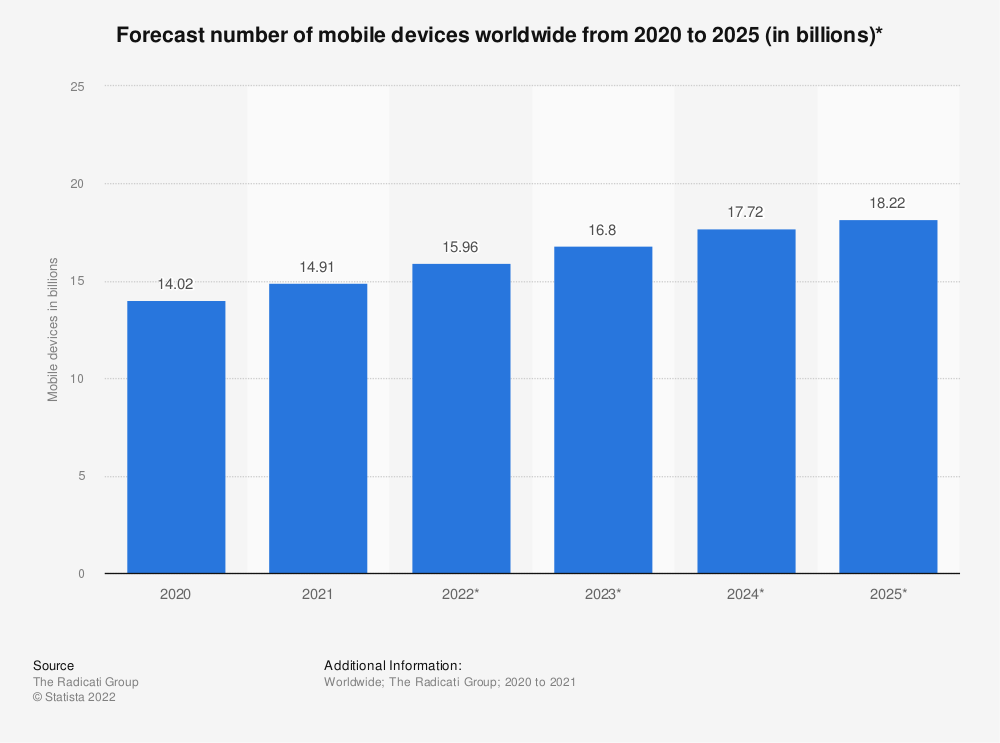
\includegraphics[width=\columnwidth]{images/mobiles20to25.png}
  \caption{Previsão do número de dispositivos móveis em todo o mundo de 2020 a 2025 (em bilhões)}
  \label{fig:mobiles20to25}
\end{figure}

Visto esse crescimento no uso de \acp{dm}, é perceptível que a demanda por \textbf{desenvolvimento de \textit{software}} para esta tecnologia também está aumentando. Essas soluções são chamadas de aplicativos móveis, o qual será abordado com mais detalhes na seção \ref{sec:apps} e posteriormente detalhado sobre o mercado de desenvolvimento de aplicativos na subseção \ref{ssec:dev_apps}.

\subsection{iOS}\label{ssec:ios}
\lipsum[1]


\subsection{Android}\label{ssec:android}
\lipsum[1]


\section{Aplicativos móveis}\label{sec:apps}
\lipsum[1]


\subsection{Desenvolvimento de aplicativos}\label{ssec:dev_apps}
\lipsum[1]

\subsubsection{Desenvolvimento nativo}\label{sssec:dev_apps_nativo}
\lipsum[1]

\subsubsection{Desenvolvimento híbrido}\label{sssec:dev_apps_hibrido}
\lipsum[1]


\section{[ abordar sobre o tema do app, area que es'ta associada à agronomia, etc... ]}
\lipsum[1]

